% !TEX TS-program = pdflatex
% !TEX encoding = UTF-8 Unicode

% This is a simple template for a LaTeX document using the "article" class.
% See "book", "report", "letter" for other types of document.

\documentclass[11pt]{article} % use larger type; default would be 10pt

\usepackage[utf8]{inputenc} % set input encoding (not needed with XeLaTeX)

%%% Examples of Article customizations
% These packages are optional, depending whether you want the features they provide.
% See the LaTeX Companion or other references for full information.

%%% PAGE DIMENSIONS
\usepackage{geometry} % to change the page dimensions
\geometry{a4paper} % or letterpaper (US) or a5paper or....
% \geometry{margin=2in} % for example, change the margins to 2 inches all round
% \geometry{landscape} % set up the page for landscape
%   read geometry.pdf for detailed page layout information

\usepackage{graphicx} % support the \includegraphics command and options

% \usepackage[parfill]{parskip} % Activate to begin paragraphs with an empty line rather than an indent

%%% PACKAGES
\usepackage[labelfont=bf,justification=centering]{caption}
\usepackage{booktabs} % for much better looking tables
\usepackage{array} % for better arrays (eg matrices) in maths
\usepackage{paralist} % very flexible & customisable lists (eg. enumerate/itemize, etc.)
\usepackage{verbatim} % adds environment for commenting out blocks of text & for better verbatim
\usepackage{subfig} % make it possible to include more than one captioned figure/table in a single float
% These packages are all incorporated in the memoir class to one degree or another...

%%% HEADERS & FOOTERS
\usepackage{fancyhdr} % This should be set AFTER setting up the page geometry
\pagestyle{fancy} % options: empty , plain , fancy
\renewcommand{\headrulewidth}{0pt} % customise the layout...
\lhead{}\chead{}\rhead{}
\lfoot{}\cfoot{\thepage}\rfoot{}

%%% SECTION TITLE APPEARANCE
\usepackage{sectsty}
\allsectionsfont{\sffamily\mdseries\upshape} % (See the fntguide.pdf for font help)
% (This matches ConTeXt defaults)

%%% ToC (table of contents) APPEARANCE
\usepackage[nottoc,notlof,notlot]{tocbibind} % Put the bibliography in the ToC
\usepackage[titles,subfigure]{tocloft} % Alter the style of the Table of Contents
\renewcommand{\cftsecfont}{\rmfamily\mdseries\upshape}
\renewcommand{\cftsecpagefont}{\rmfamily\mdseries\upshape} % No bold!

%%% END Article customizations

%%% The "real" document content comes below...

\title{MLViz: How to guide}
\date{} % Activate to display a given date or no date (if empty),
         % otherwise the current date is printed 

\begin{document}
\maketitle

MLViz is a suite of interactive visualisation tools to assist the exploratory analysis of high-dimensional datasets. It is based on the Bokeh and sci-kit learn libraries and is developed to integrate directly with Jupyter notebooks so it can be used in with exisiting exploratory analysis workflows. 

This document introduces the tools (as of V0.1) and has some hints on how to use the tools.

\section{The Univariate feature selection tool}

The feature selection tool computes univariate statistical tests of each feature and allows the user to select a feature subset based on these tests. When there are a large number of features it is often unfeasible to use all the features to build a machine learning model or perform exploratory analysis of and this tool can help the users prioritise the features to investigate further with the other tools in the MLviz library. 

A list of the most important features (as determined by the univariate statistical tests) can be extracted as a list (see fig. \ref{fig:UVFS_features}) so they can be directly fed into different tools in the MLViz library.

\begin{figure}[!h]
\centering
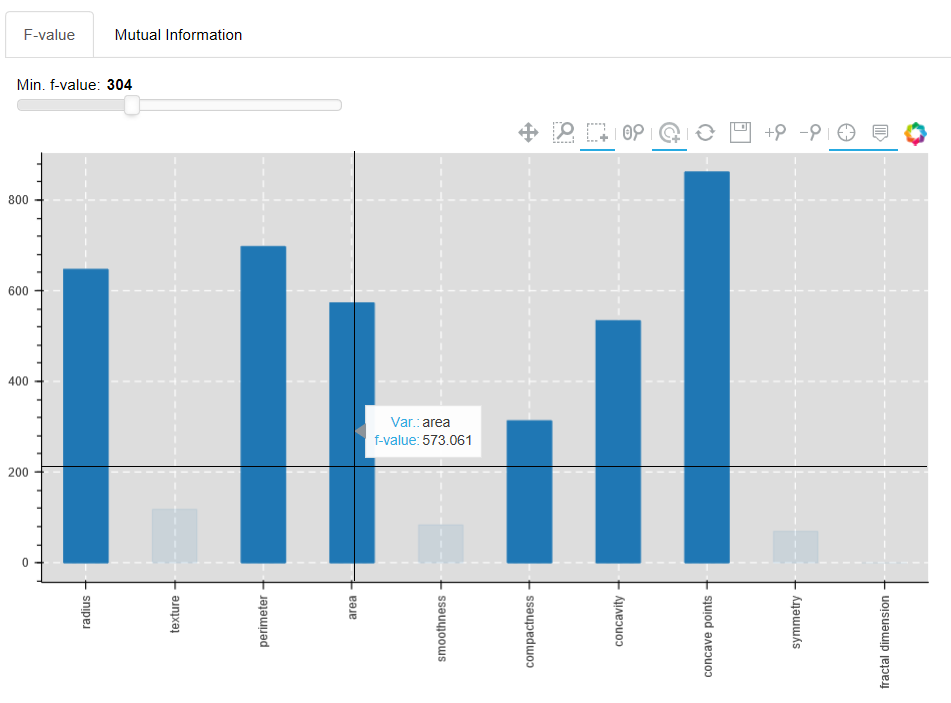
\includegraphics[width=4.5in]{images/UVFS_tool_annotated.png}
\caption{\textbf{Overview of the UVFS tool.} The horizontal axis displays each feature and the vertical axis the calculated statistical test of that feature (F-value or mutual information, shown by the highlighted tab in the top left corner). The user has the ability to select (dark shading) or de-select (light shading) using the Bokeh 'Tap tool' (Top right tool bar). A user can also threshold the features by selecting the 'minimum' value of the statistical test (using the slider, top left) to de-select features of potential low-importance.}
\label{fig:UVFS}
\end{figure}

\begin{figure}[!h]
\centering
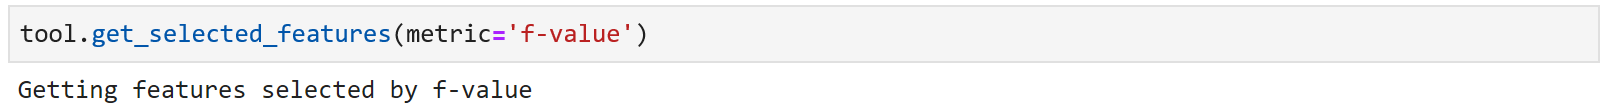
\includegraphics[width=5.75in]{images/UVFS_get_features.png}
\caption{\textbf{Extracting selected features from the UVFS tool.} This method can be used to extract the names of the features selected inthe UVFS tool (i.e., any features which are shaded in dark blue in fig. \ref{fig:UVFS}).}
\label{fig:UVFS_features}
\end{figure}

\section{The HDViz tool}

HDViz is a tool which supports the exploratory analysis of high-dimensional datasets. It allows the user to generate a 2-dimensional representation of their dataset and extract clusters of datapoints (instances which are `close' in the high dimensional space). The extracted clusters of datapoints can then be investigated using other visualisation tools to glean insights from the data set.

\begin{figure}[!h]
\centering
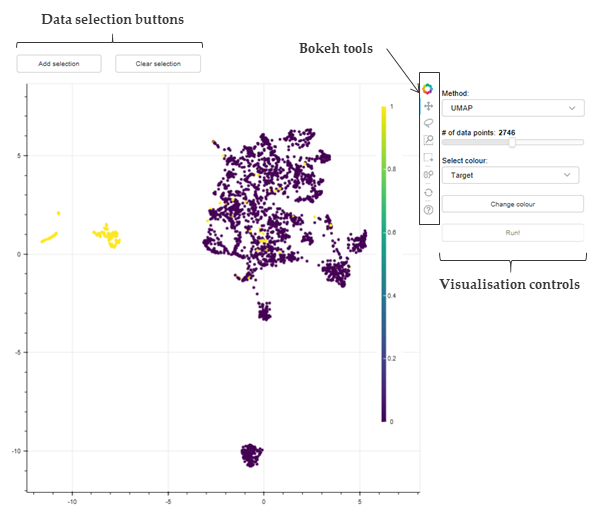
\includegraphics[width=4.5in]{images/HDViz_tool_annotated.png}
\caption{\textbf{Overview of the HDViz tool.} Graphic showing the 2-dimensional representation of the credit card data set\protect\footnote{Andrea Dal Pozzolo, Olivier Caelen, Reid A. Johnson and Gianluca Bontempi. Calibrating Probability with Undersampling for Unbalanced Classification. In Symposium on Computational Intelligence and Data Mining (CIDM), IEEE, 2015.} generated using the HDViz tool. Buttons on the right hand side are used to control the plot visualisations and parameters for performing the dimensionalty reduction and buttons along the top row are used in extracting `brushed' data.}
\label{fig:HDplot}
\end{figure}
\footnotetext{Andrea Dal Pozzolo, Olivier Caelen, Reid A. Johnson and Gianluca Bontempi. Calibrating Probability with Undersampling for Unbalanced Classification. In Symposium on Computational Intelligence and Data Mining (CIDM), IEEE, 2015.}

\subsection{Bokeh tools}

The HDViz tool is configured with standard Bokeh tools to enable the user to navigate the data, the available tools are outlined in tab. \ref{tab:bokeh_tools}. They allow the user to pan the data, zoom and select different instances of the data set.

\begin{table}[!h]
\centering
\begin{tabular}{
    >{\centering\arraybackslash}m{1cm}% instead of "p" is "m"
    |>{\centering\arraybackslash}m{12cm}
    }


\includegraphics[width=0.35in]{images/bokeh_tools_move} & \textbf{Pan:} Pan the scatter data.  \\

\includegraphics[width=0.35in]{images/bokeh_tools_lassoo} & \textbf{Lasso select:} Freely select plotted data points.\\ 

\includegraphics[width=0.35in]{images/bokeh_tools_boxzoom} & \textbf{Box zoom:} zoom on selected rectangular region.   \\

\includegraphics[width=0.35in]{images/bokeh_tools_boxselect} & \textbf{Box select:} Select data points within rectangular region. \\ 

\includegraphics[width=0.35in]{images/bokeh_tools_reset} & \textbf{Reset:} Reset the figure (i.e., remove all zooms and selections).\\ 
\end{tabular}
\caption{\textbf{The different Bokeh tools included with the HDViz tool.} The left column displays the graphic representing the tool and the right column displays its name (bold) and a short description of its function.}
\label{tab:bokeh_tools}
\end{table}

\subsection{Using the tool}

The tool is initialised by calling the HDViz class, passing it the appropiate arguments (i.e., as a minimum, the training set as a pandas dataframe), this command is shown in fig. \ref{fig:HDViz_init}. It is important to assign this class to a variable so the instance attributes of HDViz can be accessed later by the user.

\begin{figure}[!h]
\centering
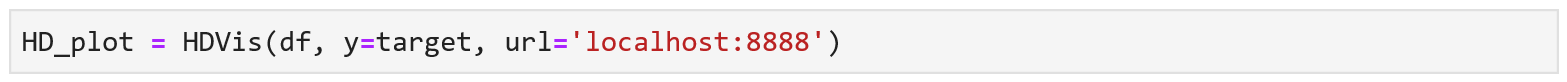
\includegraphics[width=5.75in]{images/HDViz_intialisation.png}
\caption{\textbf{Initialisation of the HDViz plot in a Jupyter notebook.} When calling the HDviz class it is important to assign it to a variable (in this case `HD\_plot'). It takes one argument as default (a pandas dataframe of the training data) but can also take the target and the location (`url' kwarg) of the notebook for output.}
\label{fig:HDViz_init}
\end{figure}

\subsubsection{Generating the low dimensional representation}

Once the plot has loaded the user will be presented with an empty figure panel with various buttons for interaction (see previous section).  To get a 2-dimensional representation of the data set the user must:

\begin{itemize}
\item Select the dimensionality reduction method to use (PCA, t-SNE or UMAP).
\item Select the number of (randomly selected) data points to embed (by default, equal to half the training set).
\item Click the `Run!' button to begin the calculation. 
\end{itemize}

The dimensionality reduction algorithms can take a long time to run and it is important to note the computational complexity for each algorthim (see appendix). A good default is the UMAP algorthim as it scales linearly with the number of training instances and generally provides fairly robust embeddings. We recommended trying an embedding with a sample of the traning set (e.g., 2500 data points) before running the full data set.


\subsubsection{Exploring and extracting data}

Once the algorithm has run successfully the `Run!' button is disabled and the figure should now look like the one displayed fig. \ref{fig:HDplot}. The user can now select to colour the data points by different features or the target (using the `Visualisation controls' located to the right hand side of the plot). Additionally, at this stage the Bokeh tools can be used to select different clusters of data points and then add them (ready for extraction) using the 'Add selection' button, located on the top row. This will append the brushes to a list so all user brushes can be accessed in the jupyter notebook in which the plot is embedded. The 'Clear selections' button removes all of the brushes previously added with the 'Add selection' button.

Once a sufficient number of brushes have been extracted (5 is a reasonable maximum number, or visualisation is inhibited) the data can be extracted by calling the `get\_user\_brushes()' method of the HDViz instance (shown in fig. \ref{fig:get_data_method}). The returned data (stored in a pandas dataframe) also have a new column `cluster\_number' which shows in which user brushing the datapoint was part of (i.e., their first, second and so on brush). This data can now be fed into other tools in the MLViz pipeline to enable

\begin{figure}
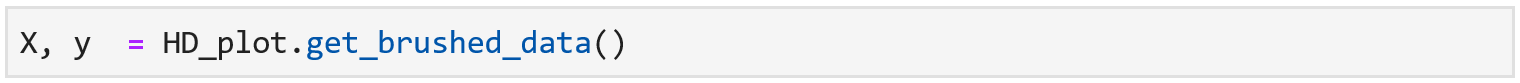
\includegraphics[width=5.75in]{images/get_brushed_data_command.png}
\caption{\textbf{Method for extracting the brushed data from the HDViz plot.} This graphic shows the method a user must call to extract the brushed data, it returns the brushed data and the targets of these brushed instances.}
\label{fig:get_data_method}
\end{figure}

\section{Draughtsman plot}

The draughtsman plot (a.k.a a pairplot) can be used in syenergy with the HDviz tool to investigate the clusters observed in the HDViz plot in the original feature space. It allows users to investigate correlations and class seperability in the original feature space.


\begin{figure}
\centering
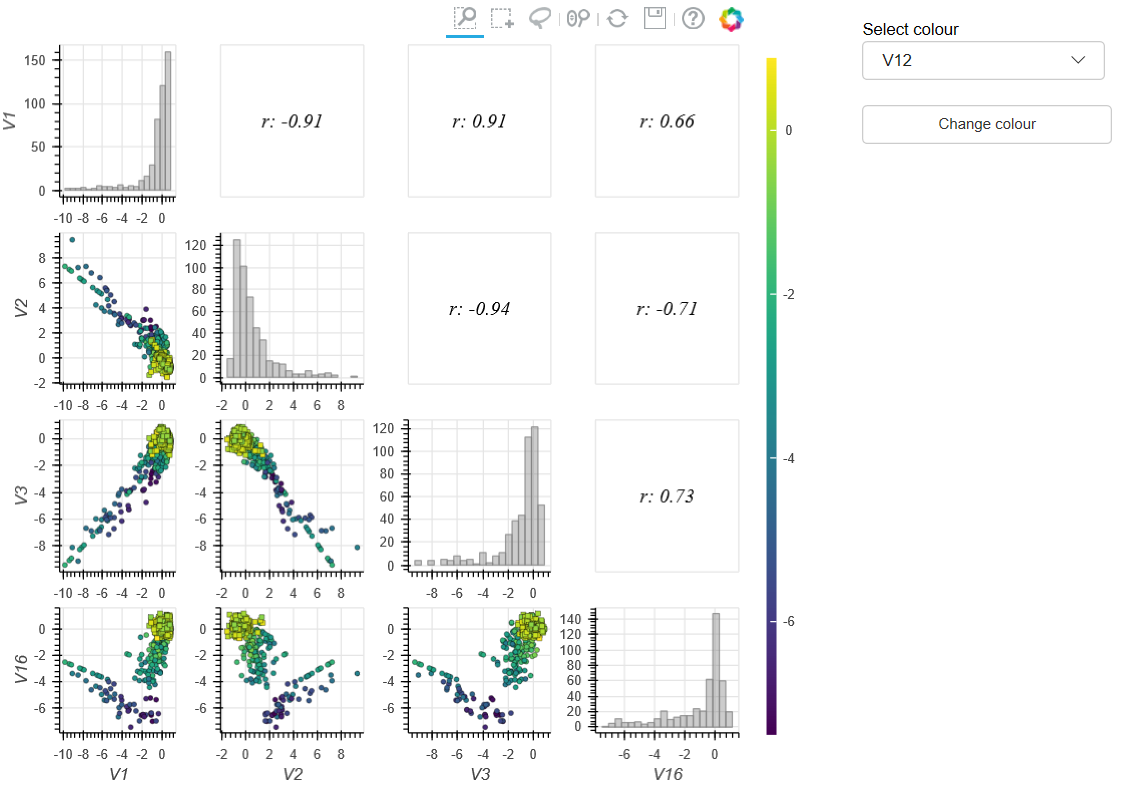
\includegraphics[width=5.75in]{images/draughtplot.png}
\caption{\textbf{The Draughtsman plot tool with example data.} Users can select which features to plot when calling the function and data points can be coloured by a user specified dimension. The upper off-diagonal panels shows the pearsons correlation coefficient for the two relevant features and the lower off-diagonals show a scatter plot of the the training instances for the two relevant features. Panels on the diagonal display a histogram training instances for the feature on the horizonal axis.}
\end{figure}

\subsection{Using the tool}

The tool is initialised by calling the DraughtPlot class, passing it the appropiate arguments (i.e., as a minimum, the training set and target values or the output of the HDViz get\_brushed\_data method), this command is shown in fig. \ref{fig:DP_init}. The user can select which features to display in the plot using the `features' kwarg, if none are provided the first five features in the training set are plotted. 

Once initialised, users can control the colour of the data points (corresponding to the values of a selected feature), zoom in and brush data points (highlighting the same instances in different panels) on the scatter plots. When brushing, the computed values (top-right off diagonal panels) are updated to reflect the metrics for the selected data points only.

\begin{figure}
\centering
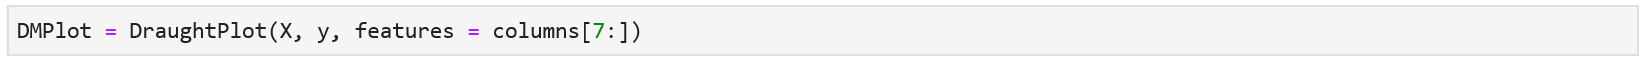
\includegraphics[width=5.75in]{images/DP_start.png}
\caption{\textbf{Initiating the Draughtsman plot.} X and y can either be the brushed data returned by the HDViz get\_brushed\_data method or the raw feature matrix and target values. The features kwarg argument is a list of features to include in the list. We recommened that the number of features is kept to approximately five or less. If a binary target (y) is provided instances with a target equal to 1 are plotted as squares and instances with a target of 0 are plotted as circles.}
\label{fig:DP_init}
\end{figure}


\clearpage

\appendix

\section{Dimensionality reduction techniques}

The HDviz tool relies upon using dimensionality reduction techniques, consistent with the sklearn API, to produce a 2-dimensional embedding of the high-dimensional dataset. There are three different methods currently implemented, all of which have different advantages and disadvantages.

\subsection{PCA}

Principle component analysis (PCA) is, arguably, the most popular dimensionality reduction technique. It works by projecting the high-dimensional data into a lower dimensional hyper plane, returning a smaller feature set whose features are a linear combination of the old features. Typically it is used to make a large feature set more managable, by lowering its dimensionality while preserving the maximum amount of variance (achieved by projecting the data into a lower dimensional hyperplane which lies closest to the data). It is not, however, that effective at embedding high-dimensional data sets into two dimensions as the information loss in discarding dimensions in the way is generally too large. It is included in MLViz as a benchmark algorthim and for rapid testing but is not generally recommend for wide-scale use.

\begin{itemize}
\item \textbf{Scalability:} Exact solution: Slow, $O(m \times n^2) + n^3$. However, Randomized PCA scales as $O(m \times d^2) + d^3$ (where $d$ is the number of dimensions to embed into and $n$ the number of features). Sklearn uses Randomized PCA automatically for large problems.
\item \textbf{Performance:} Generally performs poorly when $d$ is much less than $n$. Not practically used to visualise high-dimensional data.
\end{itemize}

\subsection{t-SNE}

t-SNE is currently the go to method for embedding high dimensional data into two dimensions, it excels in the image domain (c.f., MNIST). It generates a similarity measure between datapoints in high-dimensional space  and then distributes the datpoints in the lower dimensional space where another similarity measure is as close as possible to the high-dimensional one.

\begin{itemize}
	\item \textbf{Scalability:}  Full: $O(m \times n^2)$. But sklearn, as default, uses an approximation which scales $O(m\log(n)n)$.	
	\item \textbf{Performance:}  Known to perform well on image data sets.
\end{itemize}

\textbf{t-SNE resources:}

\begin{enumerate}
	\item L.J.P. van der Maaten and G.E. Hinton. Visualizing High-Dimensional Data Using t-SNE. Journal of Machine Learning Research 9(Nov):2579-2605, 2008
	\item Wattenberg, et al., "How to Use t-SNE Effectively", Distill, 2016. http://doi.org/10.23915/distill.00002
\end{enumerate}

\subsection{UMAP}

\textit{UMAP inherts from  sklearn classes and is therefore consistent with its API but it is not currently part of the sklearn package and is still under development. It should be considered as an experimental feature.}


UMAP is a less mature technique than t-SNE but has the potential to overtake it as the household technique for visualising high dimensional data sets. It scales much better than t-SNE, there is a direct mapping from the high-dimensional to low dimensional space and works effectively when embedding into an arbitray number of dimensions (where as t-SNE does not perform well when $m>3$).

\begin{itemize}
\item \textbf{Scalability:}  Very fast: $O(kn)$
\item \textbf{Performance:} Known to perform well on image datasets.
\end{itemize}

\textbf{UMAP resources:}

\begin{enumerate}
\item  McInnes et al., (2018). UMAP: Uniform Manifold Approximation and Projection. Journal of Open Source Software, 3(29), 861. <https://doi.org/10.21105/joss.00861>
\end{enumerate}

\end{document}
